\documentclass[aspectratio=169]{beamer}

\usetheme{Madrid}
\usecolortheme{default}

\usepackage{amsmath}
\usepackage{bm}
\usepackage{booktabs}
\usepackage{graphicx}
\usepackage{tikz}
\usepackage{animate}

\definecolor{KetteringBlue}{HTML}{1E4B99}
\setbeamercolor{structure}{fg=KetteringBlue}
\setbeamercolor{palette primary}{bg=KetteringBlue,fg=white}
\setbeamercolor{palette secondary}{bg=KetteringBlue!85!black,fg=white}
\setbeamercolor{palette tertiary}{bg=KetteringBlue!75!black,fg=white}
\setbeamercolor{frametitle}{bg=KetteringBlue,fg=white}
\setbeamercolor{title}{fg=KetteringBlue}
\setbeamercolor{block title}{bg=KetteringBlue,fg=white}
\setbeamercolor{block body}{bg=KetteringBlue!6!white,fg=black}
\setbeamercolor{headline}{bg=white,fg=KetteringBlue}
\setbeamercolor{author in head/foot}{bg=KetteringBlue,fg=white}
\setbeamercolor{date in head/foot}{bg=KetteringBlue,fg=white}

\title[Planar Rigid-Body Kinematics]{Planar Kinematics of a Rigid Body}
\subtitle{Sliding Rod Example}
\author{Esmaeil Ghorbani, Ph.D., P.Eng.}
\institute{Department of Mechanical Engineering}
\date{May 12, 2026}
% \titlegraphic{
\includegraphics[height=1.1cm]{figures/kettering_logo_converted.png}}

\newcommand{\ihat}{\hat{\imath}}
\newcommand{\jhat}{\hat{\jmath}}
\newcommand{\khat}{\hat{k}}
\newcommand{\coursename}{Planar Rigid-Body Kinematics}
\newcommand{\coursecode}{MECH 310 - Dynamics}
\newcommand{\Dknown}{\textcolor{green!50!black}{D}}
\newcommand{\Mknown}{\textcolor{green!50!black}{M}}
\newcommand{\Dunknown}{\textcolor{red!70!black}{D}}
\newcommand{\Munknown}{\textcolor{red!70!black}{M}}

\newcommand{\ketteringmark}{%
  \IfFileExists{figures/kettering_logo_converted.png}{%
    
\includegraphics[height=0.34cm]{figures/kettering_logo_converted.png}%
  }{%
    \begin{tabular}{r}
      \tiny\bfseries Kettering\\[-1.2mm]
      \tiny University
    \end{tabular}%
  }%
}

\newcommand{\constraintreferencefigure}{%
  \centering
  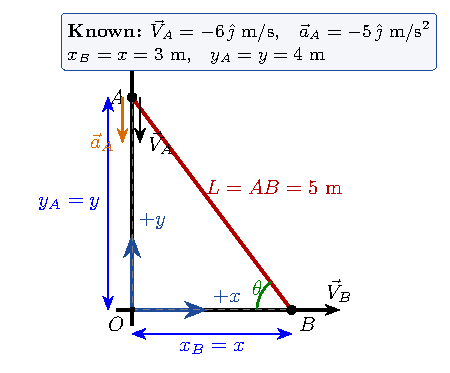
\includegraphics[width=0.72\linewidth]{figures/fig_geometric_constraint.pdf}

  \vspace{0.02cm}
  {\tiny\bfseries Coordinate convention}

  \vspace{-0.01cm}
  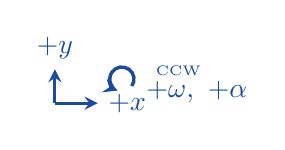
\begin{tikzpicture}[scale=0.32, >=stealth]
    \draw[->,line width=1.1pt,KetteringBlue] (0,0) -- (1.7,0)
      node[right] {$+x$};
    \draw[->,line width=1.1pt,KetteringBlue] (0,0) -- (0,1.35)
      node[above] {$+y$};
    \draw[->,line width=1.25pt,KetteringBlue]
      (3.05,0.68) arc[start angle=-35,end angle=250,radius=0.48];
    \node[KetteringBlue] at (4.9,1.3) {\tiny CCW};
    \node[KetteringBlue,anchor=west] at (3.25,0.45) {$+\omega,\ +\alpha$};
  \end{tikzpicture}%
}

\newcommand{\instantcenterreferencefigure}{%
  \centering
  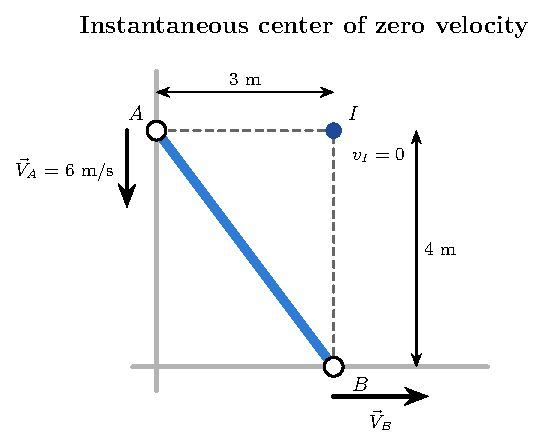
\includegraphics[width=0.82\linewidth]{figures/fig02_instantaneous_center.pdf}%
}

\newcommand{\accelerationreferencefigure}{%
  \centering
  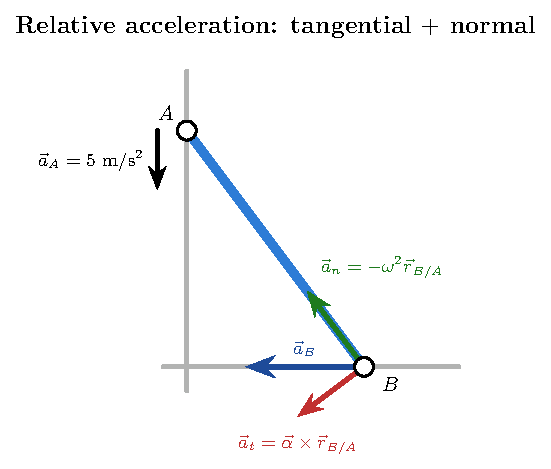
\includegraphics[width=0.64\linewidth]{figures/fig04_acceleration_components.pdf}

  \vspace{-0.08cm}
  {\tiny\itshape $\vec a_t$ shown for the solved $\alpha$; a priori
  only its line of action ($\perp \vec r_{B/A}$) is known.}%
}

\newcommand{\problemstatementfigure}[1][0.78\textwidth]{%
  \centering
  \resizebox{#1}{!}{%
    \begin{tabular}{@{}c@{}}
      \textbf{Known:}\quad
      $\vec V_A=-6\,\jhat\ \mathrm{m/s}$,\quad
      $\vec a_A=-5\,\jhat\ \mathrm{m/s^2}$\\[-0.2mm]
      $x_B=3\ \mathrm{m}$,\quad $y_A=4\ \mathrm{m}$
    \end{tabular}%
  }\par
  \vspace{0.04cm}
  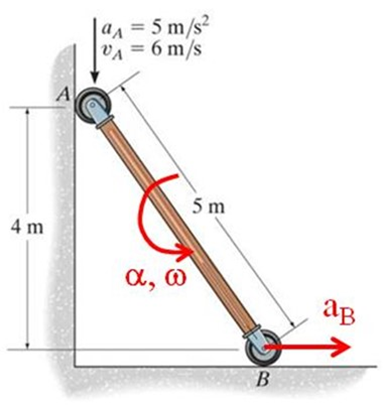
\includegraphics[width=#1]{figures/fig_problem_statement.png}%
}

\setbeamertemplate{navigation symbols}{}

\setbeamertemplate{headline}{%
  \leavevmode%
  \hbox{%
    \begin{beamercolorbox}[wd=\paperwidth,ht=0.36cm,dp=0.08cm,rightskip=0.35cm]{headline}%
      \hfill\ketteringmark
    \end{beamercolorbox}%
  }%
}

\setbeamertemplate{footline}{%
  \leavevmode%
  \hbox{%
    \begin{beamercolorbox}[wd=\paperwidth,ht=0.36cm,dp=0.15cm,leftskip=0.35cm,rightskip=0.35cm]{author in head/foot}%
      \makebox[\dimexpr\paperwidth-0.7cm\relax]{%
        \rlap{\scriptsize\coursename}%
        \hfill\scriptsize\coursecode\hfill%
        \llap{\scriptsize Esmaeil Ghorbani, Ph.D., P.Eng.\quad \insertframenumber/\inserttotalframenumber}%
      }%
    \end{beamercolorbox}%
  }%
}

\begin{document}

\begin{frame}[plain]
  \centering
  \vspace{0.5cm}
  
\includegraphics[height=1.0cm]{figures/kettering_logo_converted.png}

  \vspace{0.75cm}
  {\usebeamercolor[fg]{title}\LARGE\bfseries Planar Kinematics of a Rigid Body\par}

  \vspace{0.25cm}
  {\Large Sliding Rod Example\par}

  \vspace{0.75cm}
  {\large Esmaeil Ghorbani, Ph.D., P.Eng.\par}

  \vspace{0.2cm}
  {Department of Mechanical Engineering\par}
  {}

  \vfill
  {\small MECH 310 - Dynamics \hspace{0.5cm} May 12, 2026\par}
\end{frame}

\begin{frame}{Review of Previous Lectures}
  In the previous classes, we introduced the main tools for planar rigid-body kinematics:

  \begin{columns}[T,onlytextwidth]
    \begin{column}{0.40\textwidth}
	      \begin{itemize}
	        \item<1-> geometric constraints,
	        \item<2-> relative velocity,
	        \item<3-> instantaneous centers of zero velocity,
	        \item<4-> relative acceleration.
	      \end{itemize}
	    \end{column}
		    \begin{column}{0.58\textwidth}
		      \centering
		      \only<2>{%
		        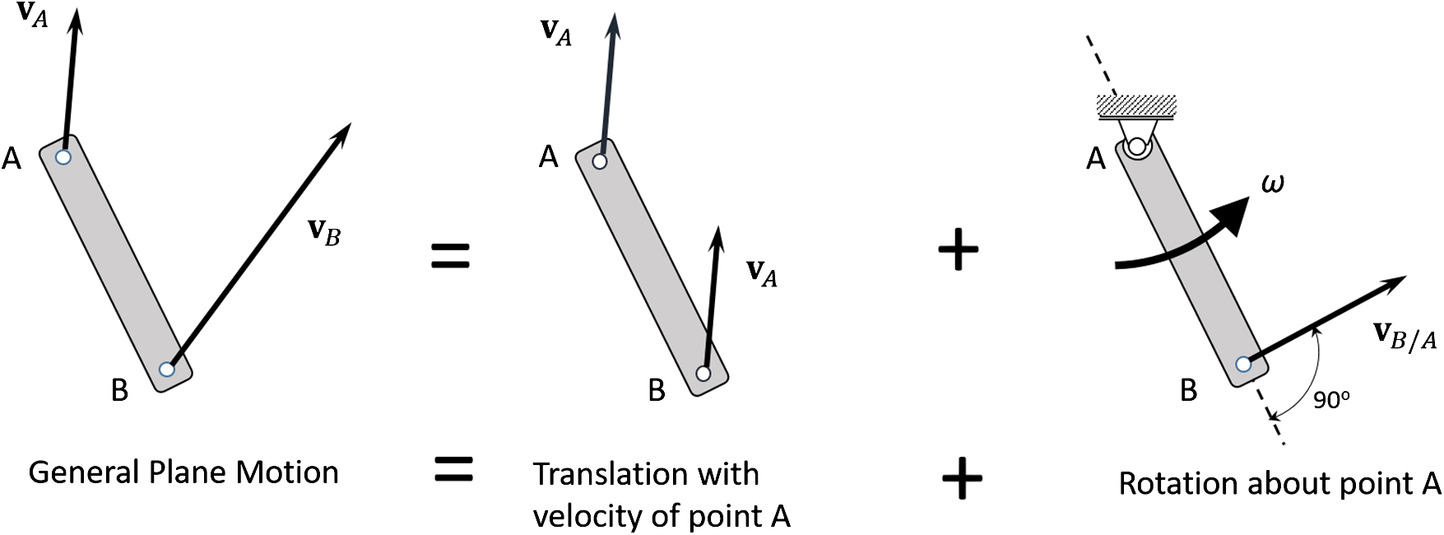
\includegraphics[width=\textwidth,height=0.54\textheight,keepaspectratio]{figures/relative_velocity.png}%
		      }
		      \only<3>{%
		        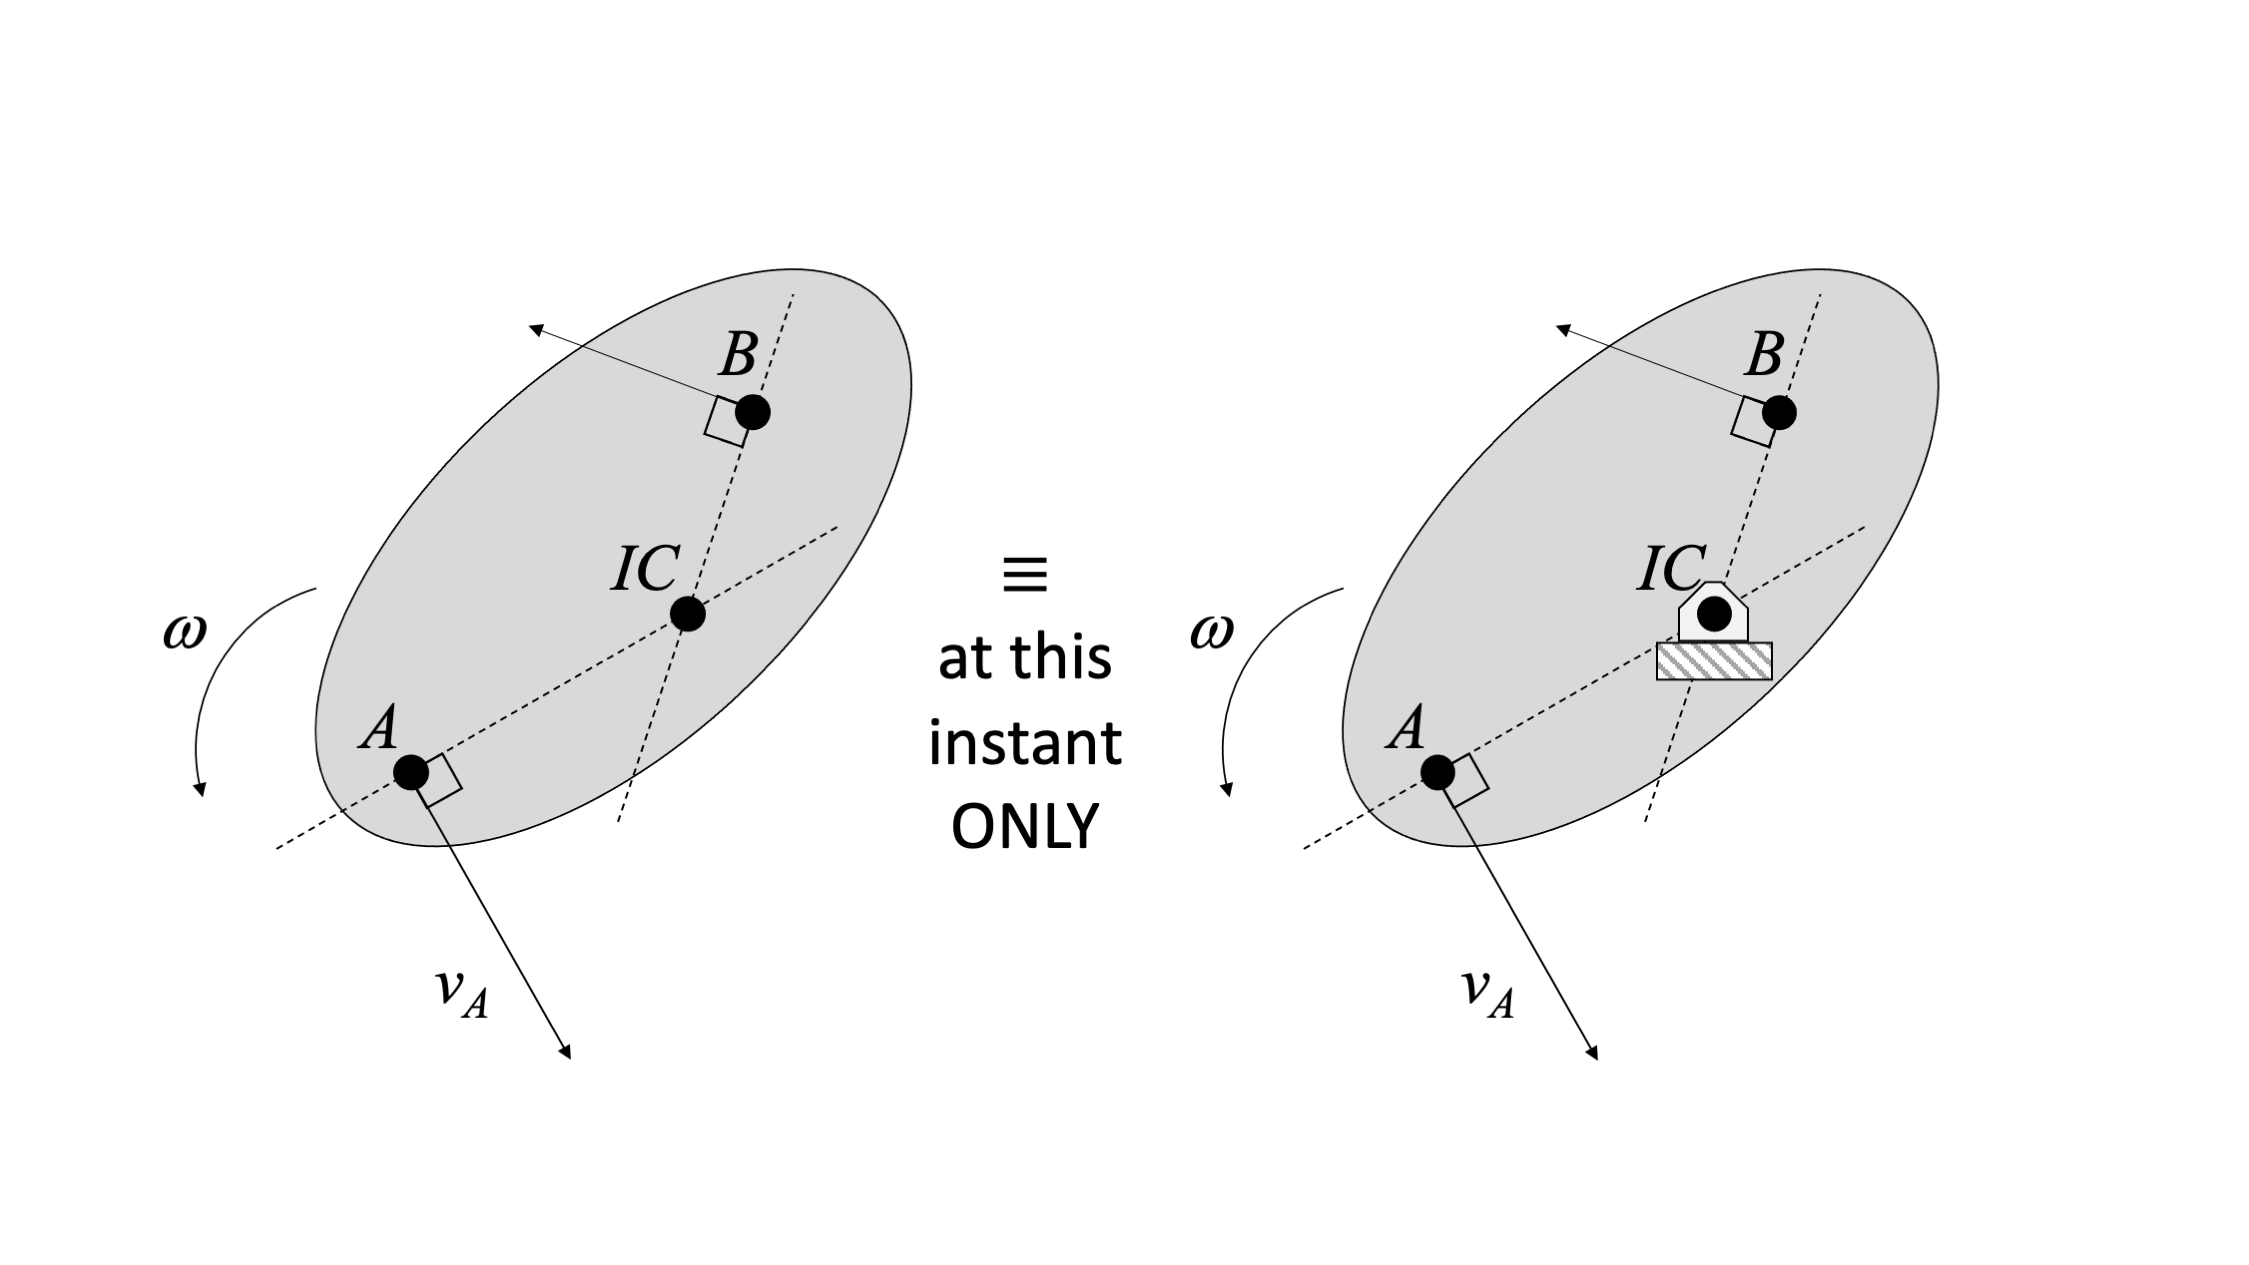
\includegraphics[width=\textwidth,height=0.54\textheight,keepaspectratio]{figures/IC3.png}%
		      }
		      \only<4>{%
		        \includegraphics[width=\textwidth,height=0.54\textheight,keepaspectratio]{\detokenize{figures/Relative acceleration.png}}%
			      }
			      \only<5->{%
			        \problemstatementfigure[0.48\textwidth]%
			      }
		    \end{column}
	  \end{columns}

	  \vspace{0.12cm}
	  \uncover<5->{%
	    \begin{center}
	      Today we use one sliding-rod problem to review all four ideas.
	    \end{center}
	  }
\end{frame}

\begin{frame}{Problem Statement}
  \begin{columns}[T,onlytextwidth]
    \begin{column}{0.52\textwidth}
      A 5 m rod has its ends constrained to slide along a vertical wall and a horizontal floor.

      \vspace{0.25cm}
      At the instant shown:
      \begin{itemize}
        \item point $A$ moves downward with speed $6\ \mathrm{m/s}$,
        \item point $A$ has acceleration $5\ \mathrm{m/s^2}$ downward,
        \item point $B$ moves horizontally,
        \item the geometry is a $3$-$4$-$5$ triangle.
      \end{itemize}

    \end{column}
    \begin{column}{0.44\textwidth}
      \problemstatementfigure[0.78\textwidth]
    \end{column}
  \end{columns}
\end{frame}

\begin{frame}{Real-World Motivation: Garage Door Motion}
  \begin{columns}[T,onlytextwidth]
    \begin{column}{0.56\textwidth}
      \centering
      \animategraphics[width=0.7\linewidth,autoplay,loop,controls]%
        {12}{figures/garage_door_frames_all/garage_all_}{000}{035}

      \vspace{0.05cm}
      {\tiny\itshape Animation plays in Adobe Acrobat.}
    \end{column}
    \begin{column}{0.40\textwidth}
      \small
      A garage door is a familiar example of constrained planar motion.

      \vspace{0.25cm}
      \begin{itemize}
        \item Rollers follow the track.
        \item Each section behaves approximately as a rigid body.
        \item The motion combines translation and rotation.
      \end{itemize}

      \vspace{0.15cm}
      This is the same kind of thinking we use for the sliding rod.
    \end{column}
  \end{columns}
\end{frame}

\begin{frame}{How the Rod Moves}
  \begin{columns}[T,onlytextwidth]
    \begin{column}{0.54\textwidth}
      \centering
      \animategraphics[width=0.7\linewidth,autoplay,loop,controls]%
        {15}{figures/motion_frames/motion_}{000}{029}

      \vspace{0.05cm}
      {\tiny\itshape Animation plays in Adobe Acrobat.}
    \end{column}
    \begin{column}{0.42\textwidth}
      \small
      \begin{itemize}
        \item Point $A$ is constrained to move only along the vertical wall.
        \item Point $B$ is constrained to move only along the horizontal floor.
        \item Since $AB$ is fixed, the rod translates and rotates at the same time.
      \end{itemize}

      \uncover<2->{
      At the shown instant, the rod forms a $3$-$4$-$5$ triangle:
      \[
      x_B=3\ \mathrm{m},\qquad y_A=4\ \mathrm{m},\qquad AB=5\ \mathrm{m}.
      \]
      }
    \end{column}
  \end{columns}
\end{frame}

\begin{frame}{What We Want to Find}
  \begin{columns}[T,onlytextwidth]
    \begin{column}{0.58\textwidth}
      \begin{block}{Unknowns}
        \[
        \omega,\qquad \vec V_B,\qquad \alpha,\qquad \vec a_B
        \]
      \end{block}

      \vspace{0.25cm}
      \footnotesize
      \begin{itemize}
        \item<2-> \textbf{Method 1.} Geometric constraint $\to$ $\omega, V_B, \alpha, a_B$.
        \item<3-> \textbf{Method 2.} Relative velocity $\to$ $\omega, V_B$.
        \item<4-> \textbf{Method 3.} Instantaneous center $\to$ $\omega, V_B$.
        \item<5-> \textbf{Method 4.} Relative acceleration $\to$ $\alpha, a_B$.
      \end{itemize}
    \end{column}
    \begin{column}{0.36\textwidth}
      \problemstatementfigure[0.95\textwidth]
    \end{column}
  \end{columns}
\end{frame}

\begin{frame}{Method 1: Geometric Constraint}
  \begin{columns}[T,onlytextwidth]
    \begin{column}{0.48\textwidth}
      \centering
      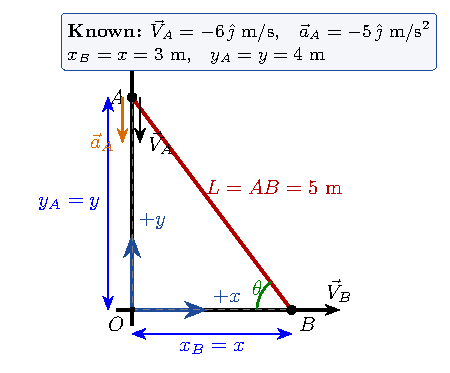
\includegraphics[width=0.58\textwidth]{figures/fig_geometric_constraint.pdf}

      \vspace{0.08cm}
      {\scriptsize\bfseries Coordinate convention}

      \vspace{0.03cm}
      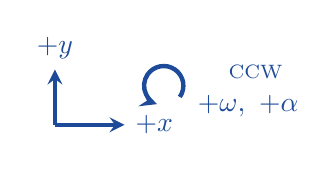
\begin{tikzpicture}[scale=0.52, >=stealth]
        \draw[->,line width=1.35pt,KetteringBlue] (0,0) -- (1.7,0)
          node[right] {$+x$};
        \draw[->,line width=1.35pt,KetteringBlue] (0,0) -- (0,1.35)
          node[above] {$+y$};
        \draw[->,line width=1.6pt,KetteringBlue]
          (3.05,0.68) arc[start angle=-35,end angle=250,radius=0.48];
        \node[KetteringBlue] at (4.9,1.3) {\scriptsize CCW};
        \node[KetteringBlue,anchor=west] at (3.25,0.45) {$+\omega,\ +\alpha$};
      \end{tikzpicture}
    \end{column}
    \begin{column}{0.48\textwidth}
      \small
      Define the variables from the triangle:
      \[
      \begin{aligned}
      x &= x_B &&= \text{horizontal position of } B,\\
      y &= y_A &&= \text{vertical position of } A,\\
      L &= AB &&= 5\ \mathrm{m}.
      \end{aligned}
      \]

      \uncover<2->{
      Since the rod length is fixed,
      \[
      \boxed{x^2+y^2=L^2}
      \]
      }

      \uncover<3->{
      At this instant:
      \[
      x=3\ \mathrm{m},\qquad y=4\ \mathrm{m}
      \]
      }
    \end{column}
  \end{columns}
\end{frame}

\begin{frame}[shrink=5]{Velocity From the Constraint}
  \begin{columns}[T,onlytextwidth]
    \begin{column}{0.58\textwidth}
      Start with:
      \[
      x^2+y^2=L^2
      \]

      \uncover<2->{
      Differentiate once:
      \[
      2x\dot{x}+2y\dot{y}=0
      \qquad\Rightarrow\qquad
      x\dot{x}+y\dot{y}=0
      \]
      }

      \uncover<3->{
      Since $\dot{y}=V_A=-6\ \mathrm{m/s}$,
      \[
      3\dot{x}+4(-6)=0
      \]
      }

      \uncover<4->{
      \[
      \boxed{\vec V_B=\dot{x}\,\ihat=8\,\ihat\ \mathrm{m/s}}
      \]
      }
    \end{column}
    \begin{column}{0.38\textwidth}
      \constraintreferencefigure
    \end{column}
  \end{columns}
\end{frame}

\begin{frame}[shrink=8]{Angular Velocity From the Geometry}
  \begin{columns}[T,onlytextwidth]
    \begin{column}{0.58\textwidth}
      \small
      Use
      \[
      x=L\cos\theta,\qquad y=L\sin\theta
      \]

      \uncover<2->{
      Differentiate $y=L\sin\theta$:
      \[
      \dot{y}=L\cos\theta\,\dot{\theta}=3\dot{\theta}
      \]
      }

      \uncover<3->{
      \[
      -6=3\dot{\theta}
      \qquad\Rightarrow\qquad
      \dot{\theta}=-2\ \mathrm{rad/s}
      \]
      }

      \uncover<4->{
      \footnotesize Note: $\theta$ is the rod-floor angle (a parameter), not the rigid-body orientation. The orientation angle of $\vec r_{B/A}$ is $-\theta$, so the rigid-body angular velocity is $\omega=-\dot\theta$.
      \normalsize
      \[
      \boxed{\omega=-\dot{\theta}=2\ \mathrm{rad/s\ CCW}}
      \]
      }
    \end{column}
    \begin{column}{0.38\textwidth}
      \constraintreferencefigure
    \end{column}
  \end{columns}
\end{frame}

\begin{frame}[shrink=5]{Acceleration From the Constraint}
  \begin{columns}[T,onlytextwidth]
    \begin{column}{0.58\textwidth}
      Differentiate the constraint a second time:
      \[
      x\ddot{x}+y\ddot{y}+\dot{x}^{2}+\dot{y}^{2}=0
      \]

      \uncover<2->{
      Substitute the known values:
      \[
      3a_B+4(-5)+(8)^2+(-6)^2=0
      \]
      }

      \uncover<3->{
      \[
      3a_B+80=0
      \]
      }

      \uncover<4->{
      \[
      \boxed{\vec a_B=-\frac{80}{3}\,\ihat\ \mathrm{m/s^2}}
      \]
      }
    \end{column}
    \begin{column}{0.38\textwidth}
      \constraintreferencefigure
    \end{column}
  \end{columns}
\end{frame}

\begin{frame}{Angular Acceleration From the Geometry}
  \begin{columns}[T,onlytextwidth]
    \begin{column}{0.58\textwidth}
      \small
      Differentiate
      \[
      \dot{y}=L\cos\theta\,\dot{\theta}
      \]

      \uncover<2->{
      \[
      \ddot{y}=-L\sin\theta\,\dot{\theta}^{2}
      +L\cos\theta\,\ddot{\theta}
      \]
      }

      \uncover<3->{
      Using $L\sin\theta=4$, $L\cos\theta=3$, $\dot{\theta}=-2$, and $\ddot{y}=-5$:
      \[
      -5=-4(2)^2+3\ddot{\theta}
      \]
      }

      \uncover<4->{
      \[
      \ddot{\theta}=\frac{11}{3}\ \mathrm{rad/s^2},
      \qquad
      \boxed{\alpha=-\frac{11}{3}\ \mathrm{rad/s^2}}
      \]
      }
    \end{column}
    \begin{column}{0.38\textwidth}
      \constraintreferencefigure
    \end{column}
  \end{columns}
\end{frame}

\begin{frame}{Motion Intuition}
  \begin{columns}[T,onlytextwidth]
    \begin{column}{0.48\textwidth}
      \begin{itemize}
        \item The rod translates and rotates at the same time.
        \item The distance between $A$ and $B$ stays constant.
        \item The wall and floor impose the motion directions.
      \end{itemize}

      \[
      \vec r_{B/A}=3\,\ihat-4\,\jhat\ \mathrm{m}
      \]
    \end{column}
    \begin{column}{0.48\textwidth}
      \centering
      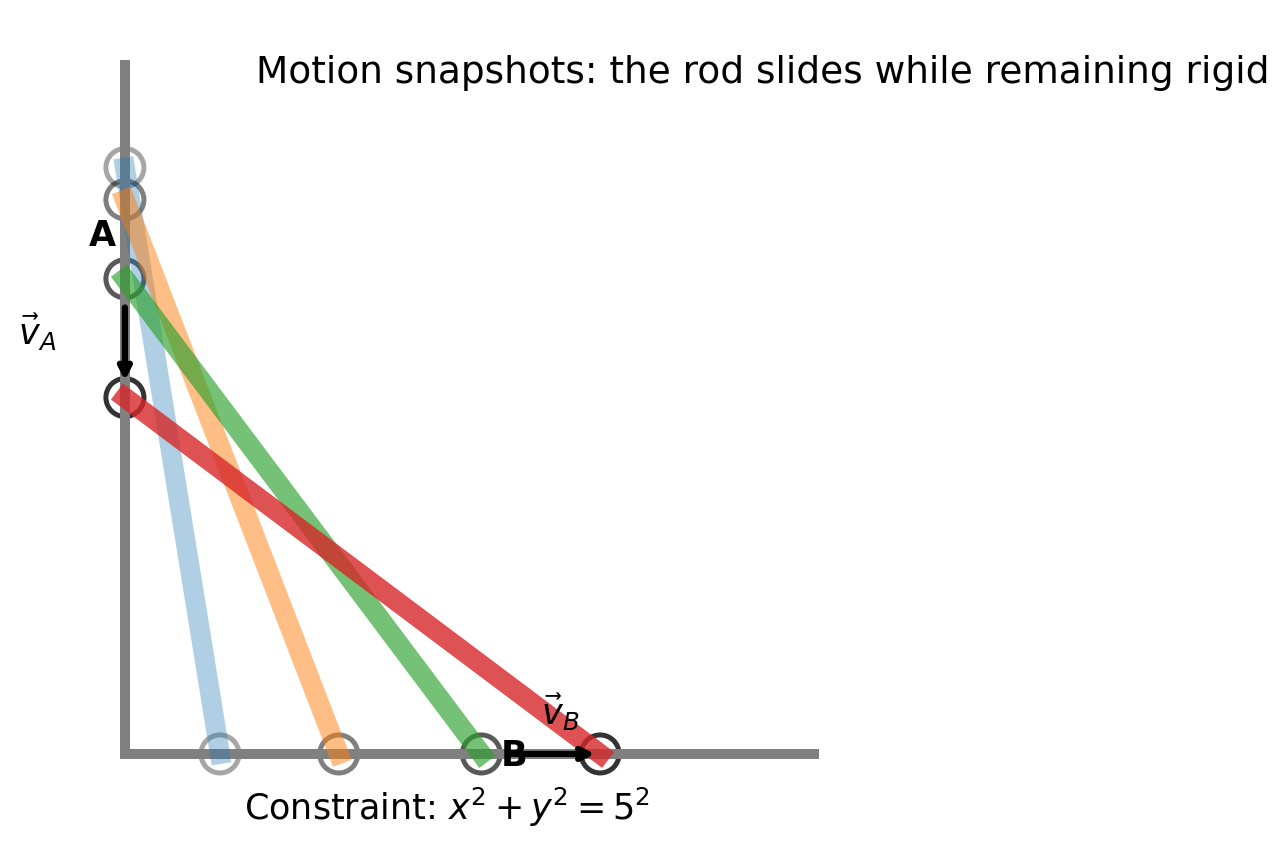
\includegraphics[width=\textwidth]{figures/fig01_motion_snapshots.png}
    \end{column}
  \end{columns}
\end{frame}

\begin{frame}{Method 2: Relative Velocity}
  \begin{columns}[T,onlytextwidth]
    \begin{column}{0.58\textwidth}
      \small
      For two points $A$ and $B$ on the same rigid body:
      \[
      \underset{
        \substack{
          \Dknown\\[0.7mm]
          \Munknown
        }
      }{\vec V_B}
      =
      \underset{
        \substack{
          \Dknown\\[0.7mm]
          \Mknown
        }
      }{\vec V_A}
      +
      \underset{
        \substack{
          \Dknown\\[0.7mm]
          \Munknown
        }
      }{\vec\omega\times\vec r_{B/A}}
      \]

      \vspace{-0.05cm}
      \scriptsize
      This vector equation gives two scalar component equations, so we can solve for two unknown magnitudes: $V_B$ and $\omega$.

      \uncover<2->{
      \vspace{-0.02cm}
      Substitute the known vectors:
      \[
      V_B\ihat=-6\jhat+\omega\khat\times(3\ihat-4\jhat)
      \]
      }

      \uncover<3->{
      \vspace{-0.08cm}
      Since
      \[
      \khat\times(3\ihat-4\jhat)=4\ihat+3\jhat,
      \]
      }

      \uncover<4->{
      \vspace{-0.08cm}
      \[
      V_B\ihat=-6\jhat+\omega(4\ihat+3\jhat)
      \]
      }
    \end{column}
    \begin{column}{0.38\textwidth}
      \constraintreferencefigure
    \end{column}
  \end{columns}
\end{frame}

\begin{frame}{Relative Velocity Result}
  \begin{columns}[T,onlytextwidth]
    \begin{column}{0.58\textwidth}
      Equating components in $V_B\hat\imath = -6\hat\jmath + \omega(4\hat\imath + 3\hat\jmath)$:
      \[
      \begin{aligned}
      \hat\imath:&\quad V_B = 4\omega \\
      \hat\jmath:&\quad 0 = -6 + 3\omega
      \end{aligned}
      \]

      \uncover<2->{
      \[
      \boxed{\omega=2\ \mathrm{rad/s\ CCW}}
      \]
      }

      \uncover<3->{
      \[
      \boxed{\vec V_B=8\,\ihat\ \mathrm{m/s}}
      \]
      }
    \end{column}
    \begin{column}{0.38\textwidth}
      \constraintreferencefigure
    \end{column}
  \end{columns}
\end{frame}

\begin{frame}{Method 3: Instantaneous Center}
  \begin{columns}[T,onlytextwidth]
    \begin{column}{0.48\textwidth}
      \centering
      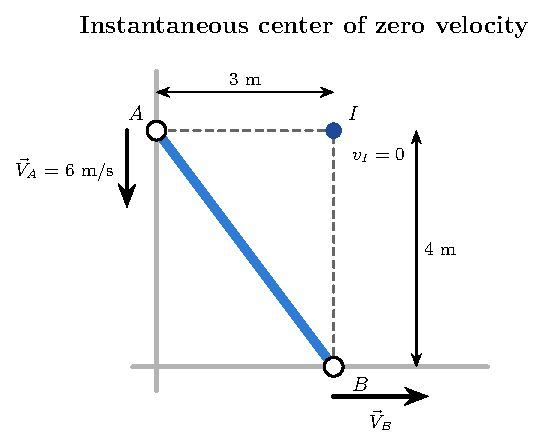
\includegraphics[width=\textwidth]{figures/fig02_instantaneous_center.pdf}
    \end{column}
    \begin{column}{0.48\textwidth}
      \begin{itemize}
        \item We know the directions of $\vec V_A$ and $\vec V_B$ from the guides.
        \item Draw a line through each point perpendicular to its velocity direction.
        \item At $A$, $\vec V_A$ is vertical, so $IA$ is horizontal.
        \item At $B$, $\vec V_B$ is horizontal, so $IB$ is vertical.
        \item The two perpendicular lines intersect at $I$, the instantaneous center.
      \end{itemize}

      \uncover<2->{
      \[
      IA=3\ \mathrm{m},\qquad IB=4\ \mathrm{m}
      \]
      }
    \end{column}
  \end{columns}
\end{frame}

\begin{frame}[shrink=8]{Instantaneous Center Result}
  \begin{columns}[T,onlytextwidth]
    \begin{column}{0.52\textwidth}
      \small
      The body rotates about $I$. Since $V_A$ is known, use point $A$ to find $\omega$:
      \[
      V_A=\omega\,IA
      \]

      \uncover<2->{
      \[
      6=\omega(3)
      \qquad\Rightarrow\qquad
      \boxed{\omega=2\ \mathrm{rad/s\ CCW}}
      \]
      }

      \uncover<3->{
      \[
      V_B=\omega\,IB=2(4)=8\ \mathrm{m/s}
      \]
      }

      \uncover<4->{
      \[
      \boxed{\vec V_B=8\,\ihat\ \mathrm{m/s}}
      \]
      }

      \uncover<5->{
      \begin{center}\scriptsize\itshape
      Cross-check: all three methods give $\omega=2$ rad/s and $V_B=8$ m/s.
      \end{center}
      }
    \end{column}
    \begin{column}{0.44\textwidth}
      \instantcenterreferencefigure
    \end{column}
  \end{columns}
\end{frame}

\begin{frame}{Velocity Field Interpretation}
  \centering
  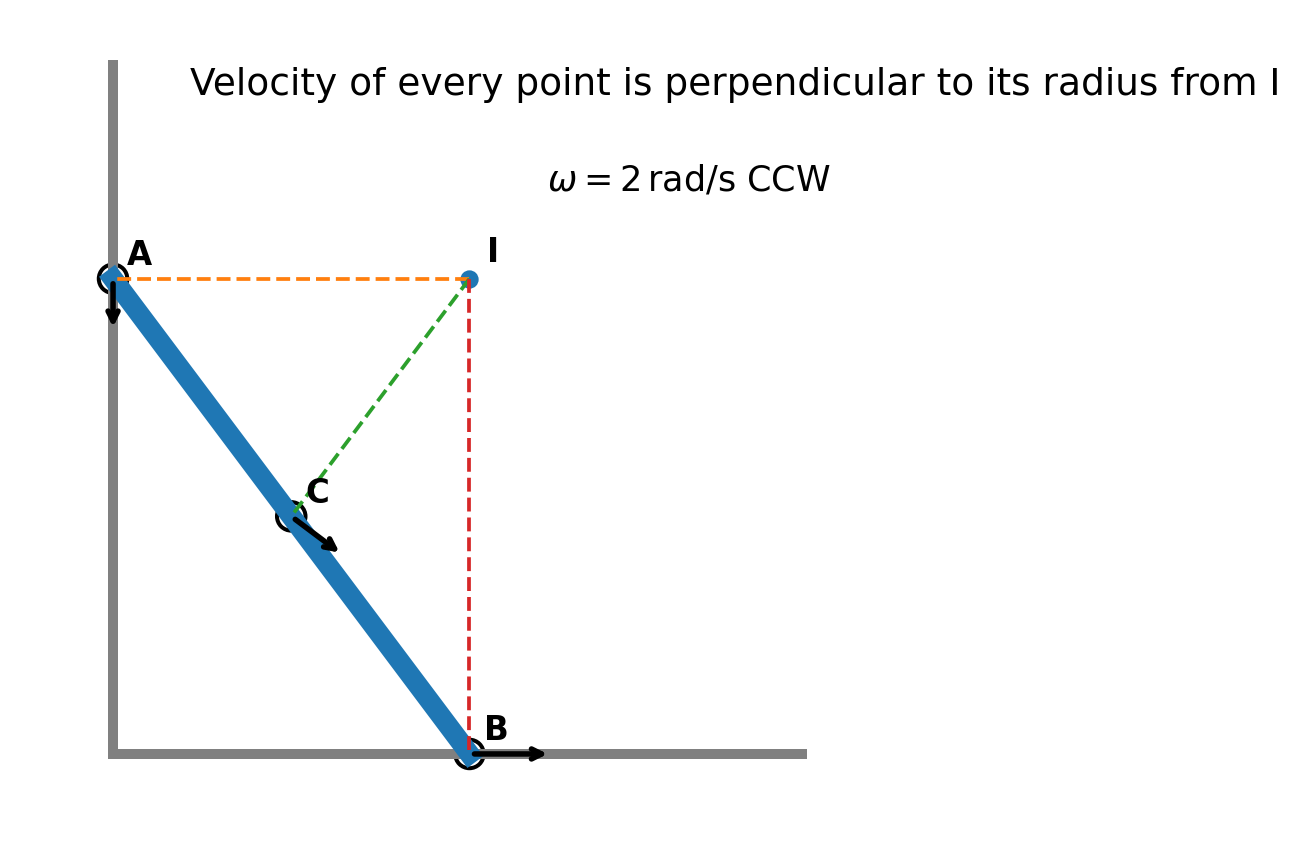
\includegraphics[height=0.68\textheight]{figures/fig03_velocity_field_from_IC.png}

  \vspace{0.2cm}
  All point velocities are perpendicular to the radius from the instantaneous center.
\end{frame}

\begin{frame}{Method 4: Relative Acceleration}
  \[
  \underset{
    \substack{
      \Dknown\\[0.7mm]
      \Munknown
    }
  }{\vec a_B}
  =
  \underset{
    \substack{
      \Dknown\\[0.7mm]
      \Mknown
    }
  }{\vec a_A}
  +
  \underset{
    \substack{
      \Dknown\\[0.7mm]
      \Munknown
    }
  }{\vec\alpha\times\vec r_{B/A}}
  -
  \underset{
    \substack{
      \Dknown\\[0.7mm]
      \Mknown
    }
  }{\omega^2\vec r_{B/A}}
  \]

  \begin{columns}[T,onlytextwidth]
    \begin{column}{0.48\textwidth}
      \uncover<2->{
      Tangential part:
      \[
      \vec a_t=\vec\alpha\times\vec r_{B/A}
      \]
      }

      \uncover<3->{
      Normal part:
      \[
      \vec a_n=-\omega^2\vec r_{B/A}
      \]
      }
    \end{column}
    \begin{column}{0.48\textwidth}
      \centering
      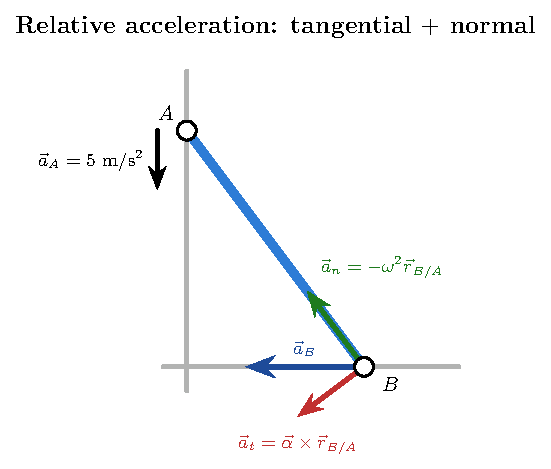
\includegraphics[width=0.66\textwidth]{figures/fig04_acceleration_components.pdf}

      \vspace{-0.1cm}
      {\scriptsize\itshape $\vec a_t$ shown for the solved $\alpha$; a priori
      only its line of action ($\perp \vec r_{B/A}$) is known.}
    \end{column}
  \end{columns}
\end{frame}

\begin{frame}{Acceleration Equation}
  \begin{columns}[T,onlytextwidth]
    \begin{column}{0.58\textwidth}
      Substitute known values:
      \[
      a_B\ihat=-5\jhat+\alpha\khat\times(3\ihat-4\jhat)
      -(2)^2(3\ihat-4\jhat)
      \]

      \uncover<2->{
      \[
      a_B\ihat=-5\jhat+\alpha(4\ihat+3\jhat)-4(3\ihat-4\jhat)
      \]
      }

      \uncover<3->{
      \[
      a_B\ihat=(4\alpha-12)\ihat+(3\alpha+11)\jhat
      \]
      }
    \end{column}
    \begin{column}{0.38\textwidth}
      \accelerationreferencefigure
    \end{column}
  \end{columns}
\end{frame}

\begin{frame}[shrink=3]{Acceleration Result}
  \begin{columns}[T,onlytextwidth]
    \begin{column}{0.58\textwidth}
      \small
      Equating components in $a_B\,\ihat=(4\alpha-12)\ihat+(3\alpha+11)\jhat$:
      \[
      \begin{aligned}
      \ihat:&\quad a_B = 4\alpha - 12 \\
      \jhat:&\quad 0 = 3\alpha + 11 \quad\text{(since $B$ stays on the floor)}
      \end{aligned}
      \]

      \uncover<2->{
      \[
      \boxed{\alpha=-\frac{11}{3}\ \mathrm{rad/s^2}}
      \]
      }

      \uncover<3->{
      \[
      a_B=4\alpha-12
      =4\left(-\frac{11}{3}\right)-12
      =-\frac{80}{3}\ \mathrm{m/s^2}
      \]
      }

      \uncover<4->{
      \[
      \boxed{\vec a_B=-\frac{80}{3}\,\ihat\ \mathrm{m/s^2}}
      \]
      }
    \end{column}
    \begin{column}{0.38\textwidth}
      \accelerationreferencefigure
    \end{column}
  \end{columns}
\end{frame}

\begin{frame}{Summary}
  \begin{columns}[T,onlytextwidth]
    \begin{column}{0.50\textwidth}
      \footnotesize
      \[
      \boxed{\omega=2\ \mathrm{rad/s\ CCW}}
      \]
      \[
      \boxed{\vec V_B=8\,\ihat\ \mathrm{m/s}}
      \]
      \[
      \boxed{\alpha=-\tfrac{11}{3}\ \mathrm{rad/s^2}
      =3.67\ \mathrm{rad/s^2\ CW}}
      \]
      \[
      \boxed{\vec a_B=-\tfrac{80}{3}\,\ihat\ \mathrm{m/s^2}
      =26.67\ \mathrm{m/s^2\ left}}
      \]

      \vspace{0.1cm}
      \scriptsize\itshape
      $\alpha$ is CW (opposite $\omega$) $\Rightarrow$ rod decelerating.\\
      $\vec a_B$ points left (opposite $\vec V_B$) $\Rightarrow$ $B$ slowing down.
    \end{column}
    \begin{column}{0.48\textwidth}
      \centering
      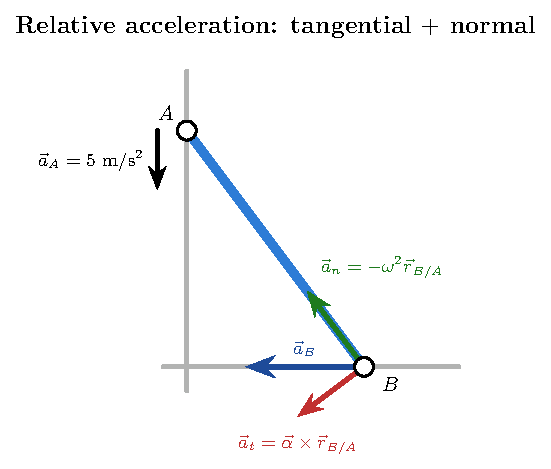
\includegraphics[width=0.80\textwidth]{figures/fig04_acceleration_components.pdf}

      \vspace{0.02cm}
      \scriptsize
      \begin{tabular}{@{}rl@{}}
      $\omega,\alpha$ & : rotation of the rod \\
      $\vec V_B,\vec a_B$ & : motion of $B$ along the floor \\
      $\vec a_n$ & : centripetal ($B \to A$) \\
      $\vec a_t$ & : tangential ($\perp$ rod)
      \end{tabular}
    \end{column}
  \end{columns}
\end{frame}

\begin{frame}{Common Pitfalls}
  \footnotesize
  \begin{itemize}
    \item \textbf{Sign of $V_A$.} ``$6$ m/s downward'' means $V_A=-6$ m/s in $\hat\jmath$ components, not $+6$.
    \item \textbf{Velocity vs.\ acceleration direction.} $\vec V$ is the direction of motion; $\vec a$ tells you accelerating ($\vec a$ along $\vec V$) or decelerating ($\vec a$ opposite $\vec V$). Opposite signs do \emph{not} mean reversal.
    \item \textbf{Parameter $\theta$ vs.\ rigid-body orientation.} If you parametrize with $x=L\cos\theta$, then $\dot\theta$ may have the opposite sign to $\omega$. Decide once which $\theta$ you mean.
    \item \textbf{Direction of $\vec a_t$.} Only its line of action ($\perp\vec r_{B/A}$) is known a priori; the sense follows from the sign of $\alpha$ \emph{after} solving.
    \item \textbf{Direction of $\vec a_n$.} Always points from $B$ toward $A$ (centripetal).
    \item \textbf{Units check.} $\omega^2|\vec r_{B/A}|$ has units $(\mathrm{rad/s})^2\cdot\mathrm{m}=\mathrm{m/s^2}$ (radians are dimensionless).
  \end{itemize}
\end{frame}

\begin{frame}{Key Takeaways}
  \begin{columns}[T,onlytextwidth]
    \begin{column}{0.52\textwidth}
      \centering
      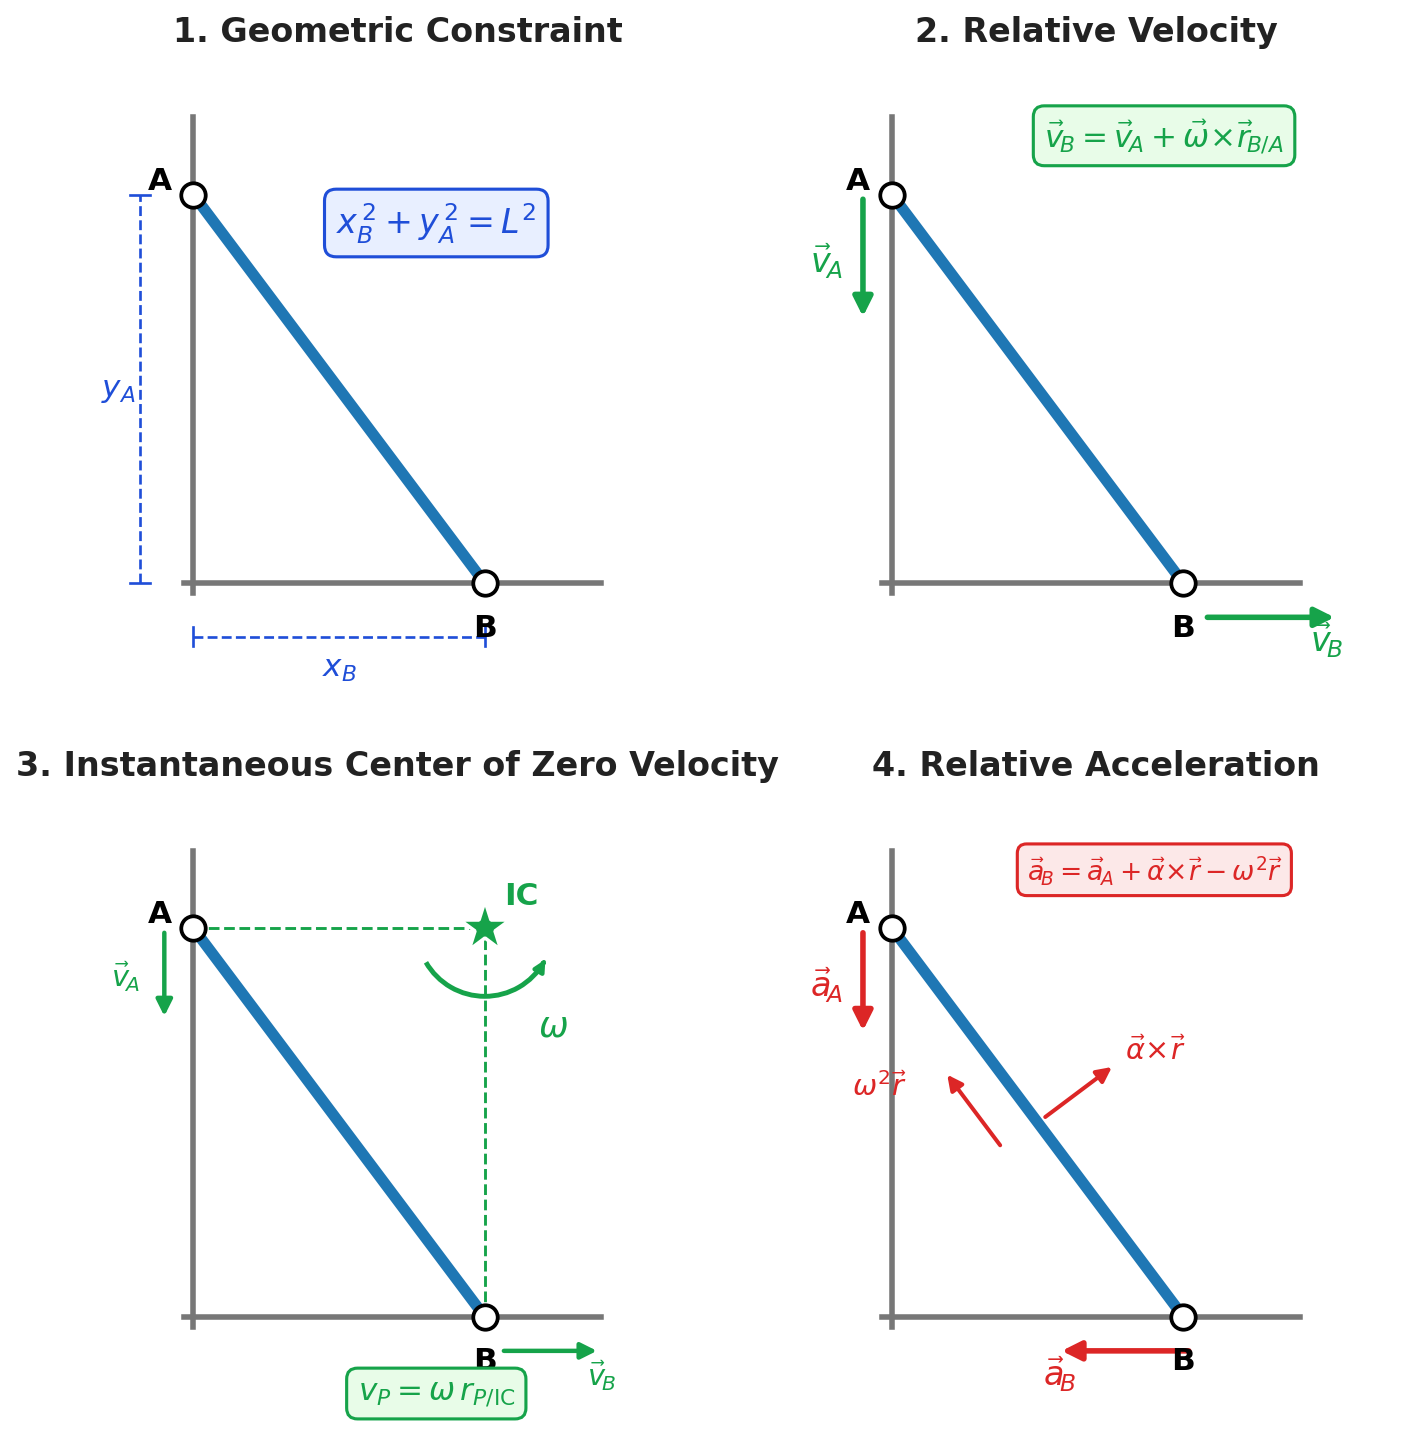
\includegraphics[height=0.78\textheight]{figures/review_overview.png}
    \end{column}
    \begin{column}{0.46\textwidth}
      \scriptsize
      \begin{enumerate}
        \item \textbf{Geometric constraint:}\\ $x_B^2 + y_A^2 = L^2$\\
              Direct route to $\omega, V_B, \alpha, a_B$.
        \item \textbf{Relative velocity:}\\ $\vec V_B = \vec V_A + \vec\omega \times \vec r_{B/A}$\\
              Systematic vector method.
        \item \textbf{Instantaneous center:}\\ $v_P = \omega\,r_{P/IC}$\\
              Visual interpretation of velocity.
        \item \textbf{Relative acceleration:}\\ $\vec a_B = \vec a_A + \vec\alpha \times \vec r - \omega^2 \vec r$\\
              Tangential $+$ normal split.
      \end{enumerate}
    \end{column}
  \end{columns}
\end{frame}

\begin{frame}{Design Question}
  \begin{columns}[T,onlytextwidth]
    \begin{column}{0.46\textwidth}
      \centering
      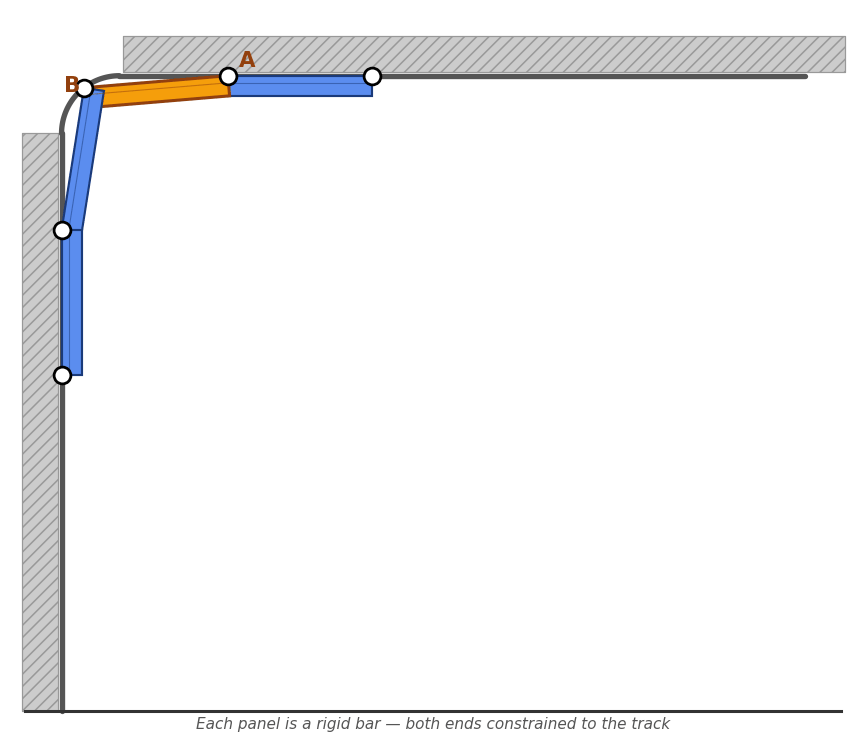
\includegraphics[width=0.62\textwidth]{figures/garage_door_frames/garage_002.png}
    \end{column}
    \begin{column}{0.50\textwidth}
      \footnotesize
      \textbf{Why is the garage-door track curved instead of a sharp corner?}

      \vspace{0.12cm}
      \begin{itemize}
        \item A sharp corner would change the velocity direction almost instantly.
        \item That would require very large angular acceleration $\alpha$.
        \item Large $\alpha$ means large required torque: $\tau \sim I\alpha$.
        \item A smooth curve keeps $\omega$, $\alpha$, roller forces, and motor torque manageable.
      \end{itemize}

      \vspace{0.05cm}
      \textbf{Design link:} these kinematic calculations help engineers size motors, rollers, and track curvature.
    \end{column}
  \end{columns}
\end{frame}

\begin{frame}{Practice: Theory, Compute and Visualize}
  \begin{columns}[T,onlytextwidth]
    \begin{column}{0.56\textwidth}
      \footnotesize
      As homework, write or complete a Python/MATLAB script that:

      \vspace{0.12cm}
      \begin{itemize}
        \item defines the rod length $L$,
        \item varies $y_A(t)$,
        \item computes
          \[
          x_B(t)=\sqrt{L^2-y_A^2(t)},
          \]
        \item computes $V_B(t)$ and $a_B(t)$,
        \item plots the rod motion and velocity.
      \end{itemize}

      \vspace{0.1cm}
      \begin{block}{Task}
        Use the geometric constraint to animate the sliding rod and plot
        $x_B(t)$, $V_B(t)$, and $a_B(t)$. Then explain where acceleration
        becomes large and why.
      \end{block}
    \end{column}
    \begin{column}{0.40\textwidth}
      \centering
      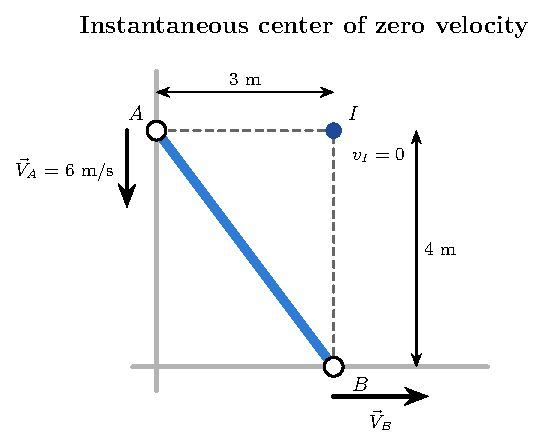
\includegraphics[width=0.82\linewidth,trim=0 0 0 0.75cm,clip]{figures/fig02_instantaneous_center.pdf}
    \end{column}
  \end{columns}
\end{frame}

\begin{frame}[shrink=8]{Check the Sign Convention}
  \begin{columns}[T,onlytextwidth]
    \begin{column}{0.7\textwidth}
      \footnotesize
      The first step in any kinematics problem is to define the coordinate system.
      Signs are not absolute; they come from the positive directions we choose.
      Do not forget the right-hand rule when defining positive rotation and the
      $+\khat$ direction.

      \vspace{0.15cm}
      \begin{block}{Student Work}
        A student used
        \[
        \vec V_A=+6\,\jhat
        \]
        and found
        \[
        \vec V_B=-8\,\ihat.
        \]
        Why?
      \end{block}

      \vspace{0.18cm}
      \uncover<2->{
      \textbf{Discussion point:} With our coordinate convention, $+\jhat$ is upward.
      Since $A$ is moving downward,
      \[
      \vec V_A=-6\,\jhat.
      \]
      The student used the opposite sign, so the computed direction of $\vec V_B$ was reversed.
      }
    \end{column}
    \begin{column}{0.38\textwidth}
      \constraintreferencefigure
    \end{column}
  \end{columns}
\end{frame}

\begin{frame}{Before You Leave}
  \footnotesize
  Answer \textbf{one} of these questions in one or two sentences:

  \vspace{0.25cm}
  \begin{enumerate}
    \item Explain why acceleration of $B$ can point left while velocity of $B$ points right.
    \item Which method do you trust most for velocity: constraint, relative velocity, or instantaneous center? Why?
  \end{enumerate}

  \vspace{0.45cm}
  \begin{center}
    \Large\textcolor{KetteringBlue}{Take care, and see you next class.\\
    Next time: rotating coordinate systems and the Coriolis effect.}
  \end{center}
\end{frame}

\end{document}
